% Generated by render_manuscript_artifacts.py from campaign root code/output_overhaul_20260601


\begin{figure}[t]
\centering
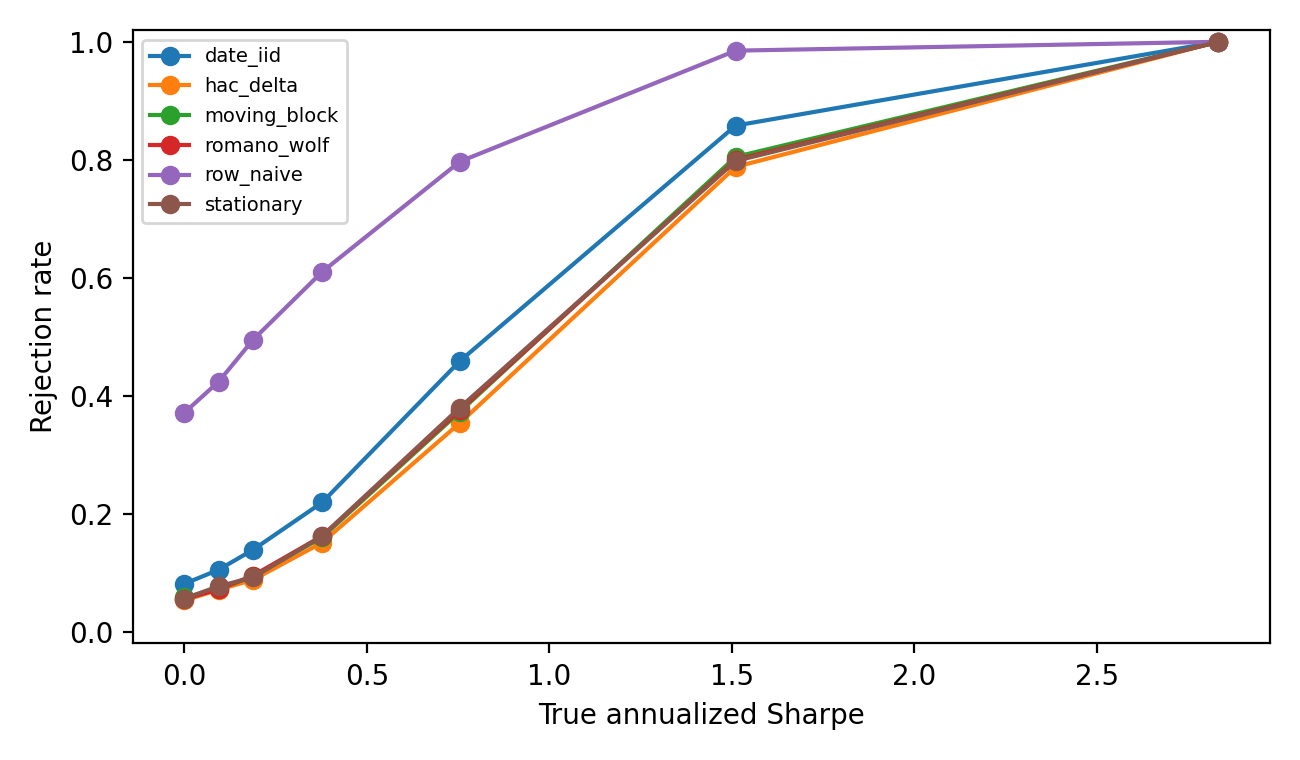
\includegraphics[width=0.82\textwidth]{generated_figures/power_curve.png}
\caption{Monte Carlo rejection rates by true annualized Sharpe.}
\label{fig:power-curve}
\end{figure}

\begin{table}[t]
\centering
\small
\caption{Simulation DGP parameter grid.}
\label{tab:dgp-grid}
\resizebox{\textwidth}{!}{%
\begin{tabular}{llllllllllll}
\toprule
DGP & Name & T & N & mu & sigma & AR1 & rho & GARCH a & GARCH b & K & regime \\
\midrule
01\_iid & IID baseline & 1000 & 50 & 4.00e-04 & 0.015 & 0.000 & 0.000 & 0.000 & 0.000 & 1 & no \\
02\_ser\_mild & Serial mild & 1000 & 50 & 4.00e-04 & 0.015 & 0.200 & 0.000 & 0.000 & 0.000 & 1 & no \\
03\_ser\_strong & Serial strong & 1000 & 50 & 4.00e-04 & 0.015 & 0.500 & 0.000 & 0.000 & 0.000 & 1 & no \\
04\_xs\_mild & Cross mild & 1000 & 50 & 4.00e-04 & 0.015 & 0.000 & 0.200 & 0.000 & 0.000 & 1 & no \\
05\_xs\_strong & Cross strong & 1000 & 50 & 4.00e-04 & 0.015 & 0.000 & 0.500 & 0.000 & 0.000 & 1 & no \\
06\_both\_mod & Both moderate & 1000 & 50 & 4.00e-04 & 0.015 & 0.200 & 0.200 & 0.000 & 0.000 & 1 & no \\
07\_both\_strong & Both strong & 1000 & 50 & 4.00e-04 & 0.015 & 0.500 & 0.500 & 0.000 & 0.000 & 1 & no \\
08\_realistic & Realistic & 2500 & 100 & 4.00e-04 & 0.015 & 0.150 & 0.350 & 0.000 & 0.000 & 1 & no \\
09\_garch\_mild & GARCH mild & 1000 & 50 & 4.00e-04 & 0.015 & 0.200 & 0.200 & 0.050 & 0.900 & 1 & no \\
10\_garch\_strong & GARCH strong & 1000 & 50 & 4.00e-04 & 0.015 & 0.300 & 0.400 & 0.100 & 0.850 & 1 & no \\
11\_multifactor & Multi-factor K=3 & 1000 & 50 & 4.00e-04 & 0.015 & 0.200 & 0.300 & 0.000 & 0.000 & 3 & no \\
12\_regime & Regime-switching & 2000 & 50 & 4.00e-04 & 0.015 & 0.150 & 0.250 & 0.000 & 0.000 & 1 & yes \\
13\_high\_ar1 & High-persistence AR(1) & 1000 & 50 & 4.00e-04 & 0.015 & 0.700 & 0.300 & 0.000 & 0.000 & 1 & no \\
14\_garch\_highvol & High-volatility GARCH & 1000 & 50 & 4.00e-04 & 0.015 & 0.200 & 0.300 & 0.150 & 0.800 & 1 & no \\
\bottomrule
\end{tabular}%
}
\end{table}

\begin{table}[t]
\centering
\small
\caption{Monte Carlo 95 percent interval coverage.}
\label{tab:coverage}
\resizebox{\textwidth}{!}{%
\begin{tabular}{llllll}
\toprule
DGP & blocked & hac\_delta & iid & row\_naive & stationary \\
\midrule
01\_iid & 0.947 & 0.952 & 0.951 & 0.000 & 0.947 \\
02\_ser\_mild & 0.938 & 0.943 & 0.898 & 0.000 & 0.936 \\
03\_ser\_strong & 0.921 & 0.934 & 0.734 & 0.000 & 0.919 \\
04\_xs\_mild & 0.950 & 0.950 & 0.952 & 0.073 & 0.950 \\
05\_xs\_strong & 0.934 & 0.938 & 0.942 & 0.262 & 0.938 \\
06\_both\_mod & 0.937 & 0.939 & 0.898 & 0.088 & 0.936 \\
07\_both\_strong & 0.934 & 0.943 & 0.771 & 0.178 & 0.935 \\
08\_realistic & 0.937 & 0.941 & 0.901 & 0.107 & 0.937 \\
09\_garch\_mild & 0.926 & 0.940 & 0.877 & 0.110 & 0.930 \\
10\_garch\_strong & 0.926 & 0.948 & 0.862 & 0.199 & 0.927 \\
11\_multifactor & 0.937 & 0.947 & 0.895 & 0.225 & 0.940 \\
12\_regime & 0.929 & 0.934 & 0.890 & 0.306 & 0.929 \\
13\_high\_ar1 & 0.899 & 0.933 & 0.562 & 0.137 & 0.907 \\
14\_garch\_highvol & 0.940 & 0.948 & 0.895 & 0.193 & 0.941 \\
\bottomrule
\end{tabular}%
}
\end{table}

\begin{table}[t]
\centering
\small
\caption{Null rejection rates at nominal 5 percent size.}
\label{tab:size}
\resizebox{\textwidth}{!}{%
\begin{tabular}{lllllll}
\toprule
dgp & date\_iid & hac\_delta & moving\_block & romano\_wolf & row\_naive & stationary \\
\midrule
null\_dep & 0.094 & 0.066 & 0.070 & 0.068 & 0.352 & 0.067 \\
null\_garch & 0.098 & 0.063 & 0.070 & 0.067 & 0.351 & 0.068 \\
null\_iid & 0.060 & 0.060 & 0.061 & 0.060 & 0.062 & 0.062 \\
\bottomrule
\end{tabular}%
}
\end{table}

\begin{table}[t]
\centering
\small
\caption{Power by true annualized Sharpe.}
\label{tab:power}
\resizebox{\textwidth}{!}{%
\begin{tabular}{llllllll}
\toprule
index & true\_sharpe & date\_iid & hac\_delta & moving\_block & romano\_wolf & row\_naive & stationary \\
\midrule
0.000 & 0.000 & 0.081 & 0.053 & 0.058 & 0.055 & 0.371 & 0.056 \\
1.000 & 0.094 & 0.105 & 0.071 & 0.072 & 0.072 & 0.424 & 0.077 \\
2.000 & 0.189 & 0.139 & 0.088 & 0.094 & 0.095 & 0.495 & 0.092 \\
3.000 & 0.378 & 0.219 & 0.151 & 0.160 & 0.162 & 0.610 & 0.162 \\
4.000 & 0.755 & 0.459 & 0.354 & 0.373 & 0.376 & 0.797 & 0.380 \\
5.000 & 1.511 & 0.858 & 0.788 & 0.805 & 0.800 & 0.985 & 0.798 \\
6.000 & 2.833 & 1.000 & 1.000 & 1.000 & 1.000 & 1.000 & 1.000 \\
\bottomrule
\end{tabular}%
}
\end{table}
